\documentclass[conference]{IEEEtran}
\IEEEoverridecommandlockouts

\usepackage{cite}
\usepackage{amsmath,amssymb,amsfonts}
\usepackage{graphicx}
\usepackage{textcomp}
\usepackage{xcolor}
\usepackage{tabularx}
\usepackage{array}
\usepackage{url}
\usepackage{tikz}

\def\BibTeX{{\rm B\kern-.05em{\sc i\kern-.025em b}\kern-.08em
    T\kern-.1667em\lower.7ex\hbox{E}\kern-.125emX}}

\newcommand{\missingfigurebox}[1]{%
    \fbox{%
        \begin{minipage}[c][0.32\linewidth][c]{0.86\linewidth}
            \centering\footnotesize Missing figure file:\\
            \texttt{\detokenize{#1}}
        \end{minipage}%
    }%
}

\newcommand{\safeincludegraphics}[2][]{%
    \IfFileExists{#2}{\includegraphics[#1]{#2}}{\missingfigurebox{#2}}%
}

\begin{document}

\title{Modeling and Simulation of Control Systems Through Block Diagrams in an Interactive Web Environment}

\author{
\IEEEauthorblockN{Vitor Silva do Nascimento, Marcus Vinicius Ara\'ujo Fernandes, Kevin Gabriel Pinheiro Castro, Vinn\'icius Alex Melo Peixoto, Calebe Freitas da Silva}
\IEEEauthorblockA{\textit{Directorate of Industry, Natal-Central Campus}\\
\textit{Federal Institute of Education, Science and Technology of Rio Grande do Norte (IFRN)}\\
Natal, RN, Brazil\\
vitrsn@gmail.com; marcus.fernandes@ifrn.edu.br; k.g.pinheiro.castro@gmail.com; vinicius.alex.melo@hotmail.com; calebe8839@gmail.com}
}

\maketitle

\begin{abstract}
Control systems engineering education requires seamless integration between mathematical abstraction and practical experimentation. Although Python scripts have expanded access to computational tools, syntax barriers may increase initial cognitive load. This paper presents the evolution of a web-based educational tool into an interactive modeling ecosystem based on block diagrams. Developed in Python with the Streamlit library, the solution removes licensing barriers and provides a responsive open-source interface. The architecture enables topological system composition and supports rigorous time- and frequency-domain analyses, including step response, Bode plots, root locus, and Nyquist diagrams. Technical accuracy was validated through a hard disk drive positioning benchmark. In addition, an exploratory user evaluation with ten participants indicated high pedagogical acceptance, with an average Likert score of 4.06, and satisfactory usability, with a System Usability Scale score of 75.5 after consistency filtering. The results show that the block-based interface and dynamic visualization reduce cognitive load and support hypothesis validation and controller design. The platform therefore acts as a pedagogical facilitator in the context of information and communication technologies, promoting a user experience that improves control systems learning.
\end{abstract}

\begin{IEEEkeywords}
Control systems education, computer-aided education, modeling and simulation, graphical systems modeling, interactive web interface.
\end{IEEEkeywords}

\section{Introduction}

Control engineering education is grounded in the modeling and simulation of dynamic systems \cite{dorf2017}. In the context of Education 5.0, information and communication technologies (ICTs) seek to promote training centered on the autonomous solution of complex problems \cite{cordeiro2024}. However, the practical implementation of these concepts still faces infrastructure challenges and limitations in access to computational environments \cite{fujiwara1992}.

Although Python is a predominant language in the scientific ecosystem \cite{reznichenko2025}, strict reliance on scripts can increase cognitive load. According to Cognitive Load Theory \cite{SWELLER2024102423}, managing complex syntax while learning new concepts can overload working memory \cite{santos2024,oliveira2025}. In parallel, proprietary software introduces financial and portability barriers \cite{manathunga2025}.

Table~\ref{tab:comparison} summarizes the limitations of current tools with respect to cost, graphical user interface (GUI), visual modeling, mobile support, and analysis capabilities. A technological gap can be observed in the combination of flexible topological modeling and cross-platform accessibility.

\begin{table}[htbp]
\caption{Comparison of tools for control systems education.}
\label{tab:comparison}
\centering
\renewcommand{\arraystretch}{1.3}
\setlength{\tabcolsep}{2pt}
\scriptsize
\begin{tabularx}{\linewidth}{@{}p{1.9cm}*{5}{>{\centering\arraybackslash}X}@{}}
\hline
\textbf{Tool} & \textbf{Cost} & \textbf{GUI} & \textbf{Blk.$^1$} & \textbf{Mob.$^2$} & \textbf{An.$^3$} \\ \hline
Simulink              & Paid          & Yes          & Yes          & No           & Yes          \\
LabVIEW               & Paid          & Yes          & Yes          & No           & Yes          \\
Python Control$^a$    & Free          & No           & No           & No           & Yes          \\
Collimator$^a$        & Free$^*$      & Yes          & Yes          & Partial      & Yes          \\
PyCSBtool$^b$         & Free          & Yes          & No           & No           & Partial      \\
LabVCon$^c$           & Free          & Yes          & --           & --           & No           \\
\textbf{CSS (Prop.)}  & \textbf{Free} & \textbf{Yes} & \textbf{Yes} & \textbf{Yes} & \textbf{Yes} \\ \hline
\end{tabularx}

\vspace{1mm}
\scriptsize
\textbf{Legend:} Blk.: block diagrams; Mob.: mobile support; An.: time/frequency analyses. \\
$^*$Limited resources. $^a$\cite{reznichenko2025}; $^b$\cite{manathunga2025}; $^c$\cite{araujo2022}.
\end{table}

This paper presents an interactive web architecture based on the Streamlit library. Unlike static assistants \cite{nascimento2025}, the proposed solution uses an engine that converts graphical compositions into mathematical models. The main contributions of this work are: (i) a graph-based pipeline for topological interpretation; (ii) a responsive interface focused on reducing cognitive load; and (iii) validation of numerical accuracy and user acceptance. This pedagogical hypothesis is investigated through an exploratory evaluation, whose results demonstrate the potential of the application as a support tool for teaching. The remainder of the paper details the architecture in Section~II, the technical and empirical validation in Section~III, and the conclusions in Section~IV.

\section{Materials and Methods}

The proposed architecture is based on the Python ecosystem and uses scientific libraries to implement control algorithms with accuracy comparable to proprietary software \cite{reznichenko2025,kim2023}. The methodology followed an incremental approach to transform the textual calculation assistant presented in \cite{nascimento2025} into a modeling environment based on topological and algebraic representations. This section details the interface layers, graph-based processing, and calculation engine, in addition to describing the exploratory user evaluation protocol used to assess the usability and pedagogical acceptance of the platform.

\subsection{Architecture and Operating Modes}

The current architecture expands the prototype described in \cite{nascimento2025} by integrating the processing of transfer functions (TFs) and state-space (SS) models. The system performs algorithmic conversion between models, ensuring data consistency across all analysis stages. To minimize cognitive load \cite{SWELLER2024102423}, the software provides two operating modes: Classic Mode, intended for direct definition through coefficients or matrices, and Block Diagram Mode, which enables visual topological composition.

The operational sequence shown in Fig.~\ref{fig:analysis_flowchart} establishes a logical flow that starts with interface selection and converges to a normalized configuration module. After defining the model, the user selects the excitation signal, namely impulse, step, or ramp, and the analysis domains, namely time, frequency, or stability. The calculation engine processes the interconnections and generates synchronous results such as root locus, Bode, and Nyquist diagrams. This immediate feedback cycle is designed to reduce the gap between mathematical formalism and perception of dynamic behavior, serving as the basis for the usability evaluation conducted in this study \cite{guzman2014}.

\begin{figure}[htbp]
    \centering
    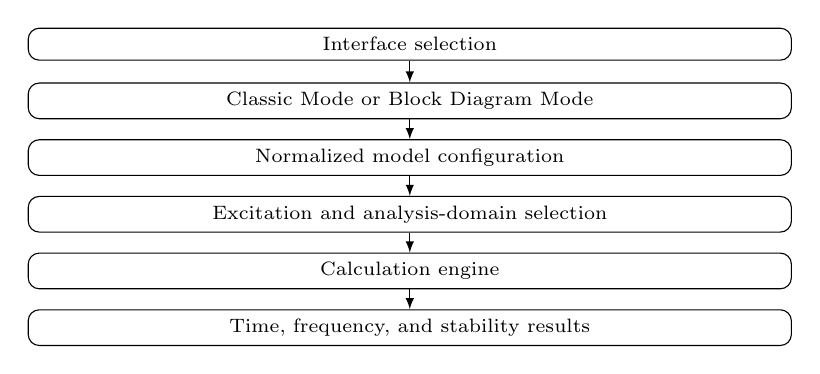
\begin{tikzpicture}[font=\scriptsize, >=latex]
        \node[draw, rounded corners, align=center, text width=0.78\linewidth] (a) at (0,0)
            {Interface selection};
        \node[draw, rounded corners, align=center, text width=0.78\linewidth] (b) at (0,-0.72)
            {Classic Mode or Block Diagram Mode};
        \node[draw, rounded corners, align=center, text width=0.78\linewidth] (c) at (0,-1.44)
            {Normalized model configuration};
        \node[draw, rounded corners, align=center, text width=0.78\linewidth] (d) at (0,-2.16)
            {Excitation and analysis-domain selection};
        \node[draw, rounded corners, align=center, text width=0.78\linewidth] (e) at (0,-2.88)
            {Calculation engine};
        \node[draw, rounded corners, align=center, text width=0.78\linewidth] (f) at (0,-3.60)
            {Time, frequency, and stability results};
        \draw[->] (a) -- (b);
        \draw[->] (b) -- (c);
        \draw[->] (c) -- (d);
        \draw[->] (d) -- (e);
        \draw[->] (e) -- (f);
    \end{tikzpicture}
    \caption{Functional architecture flowchart and operating sequence of the tool.}
    \label{fig:analysis_flowchart}
\end{figure}

\subsection{Processing Pipeline}

The proposed architecture integrates the user interface, structural interpretation, and mathematical processing into a continuous functional flow. The calculation core uses the Python-Control library to process TF and SS representations, while SymPy provides the symbolic manipulation required for model derivation and loop simplification \cite{kim2023}. Cloud execution through Streamlit ensures solution portability and removes dependencies on local hardware.

In Block Diagram Mode, the topological parser translates the graphical structure into a directed graph, algorithmically identifying series associations, parallel associations, and feedback loops. From this representation, the system synthesizes the formal mathematical model by combining symbolic operations with composition routines from Python-Control. The calculation engine uses SciPy for numerical integration and stability analysis, and the results are rendered interactively with Plotly. This pipeline ensures technical rigor and provides the immediate feedback required for hypothesis validation and the reduction of operational cognitive load \cite{guzman2014}.

\subsection{Visual Modeling Interface}

Block Diagram Mode enables the synthesis of dynamic systems through the manipulation of functional objects such as plant, controller, sensor, and actuator blocks, each parameterized by TF or SS models. The interface abstracts the algebraic complexity of matrices and polynomials by allowing the free positioning of components and their interconnection through logical ports \cite{nascimento2025}.

The editor represents system topology as a directed graph, in which blocks operate as nodes and connections as edges. The topological parser automatically identifies patterns of series association, parallel association, and feedback loops, performing block reduction to generate the equivalent closed-loop representation. This visual approach brings the academic experience closer to industrial tools and facilitates exploratory experimentation by providing immediate feedback on structural changes \cite{reznichenko2025}.

\subsection{Project Scope and Limitations}

The platform targets the domain of linear time-invariant (LTI), single-input single-output (SISO) systems. Although the architecture supports SS representations, the current simulation engine prioritizes analysis of the global input-output relationship. Consequently, multivariable systems (MIMO) and nonlinear dynamics are not addressed at this stage of development.

This delimitation is based on the need to mitigate extraneous cognitive load \cite{SWELLER2024102423}, ensuring that students focus on the fundamental concepts of classical control. By restricting the scope to moderate-order SISO systems, the environment avoids dispersing attention with the additional complexity of high-order systems, which is consistent with the principles of active learning in digital environments \cite{nascimento2025}.

Because this is a cloud-based pedagogical application, occasional processing latency is considered acceptable, since algorithmic accuracy and data integrity take precedence over real-time simulation. These definitions align with the purpose of the platform as a ubiquitous experimentation environment for theoretical modeling and practical consolidation in control engineering.

\subsection{Evaluation Methodology and Data Collection}

The tool evaluation consisted of an exploratory study with undergraduate engineering students. The experimental protocol aimed to measure pedagogical perception and software usability through a structured questionnaire organized into two dimensions: (i) Pedagogical Perception, using a 1-to-5 Likert scale focused on intuitiveness and cognitive-load reduction; and (ii) Usability, using the System Usability Scale (SUS), a validated instrument for interactive systems \cite{brooke1996sus}.

Because SUS alternates between positive and negative items, a consistency check was performed to identify response biases. Some participants showed contradictions in reverse-coded items, a phenomenon documented in the literature \cite{lewis2009factor}. To ensure reliability, the data analysis was stratified into: (i) global sample analysis and (ii) refined analysis, excluding logically inconsistent responses. This approach reduced interpretation noise in the instrument and resulted in a more reliable estimate of the platform's actual usability.

\section{Results and Discussion}

The proposed architecture was validated in two main stages: computational accuracy verification through a classical benchmark and user experience analysis. For technical validation, the hard disk drive (HDD) positioning system documented in \cite{dorf2017} was adopted because of its didactic relevance in the control of second-order systems. The open-loop transfer function is shown in \eqref{eq:dorf_system}.

\begin{equation}
G(s) = \frac{200}{s^2 + 20s + 200}
\label{eq:dorf_system}
\end{equation}

Subsections~\ref{classic_mode} and~\ref{block_mode} detail the numerical accuracy and interface responsiveness in Classic Mode and Block Diagram Mode, respectively. For the closed-loop design, the proportional-derivative (PD) controller defined in \eqref{eq:dorf_pd} was used to validate the fidelity of time and frequency responses against the design requirements of \cite{dorf2017}.

\begin{equation}
C(s) = 39.68s + 2880
\label{eq:dorf_pd}
\end{equation}

Finally, Subsection~\ref{user_validation} presents the qualitative and quantitative analysis of the application, correlating usability and pedagogical acceptance scores with the cognitive-load reduction hypothesis.

\subsection{Classic Mode Analysis and Mobile Usability}
\label{classic_mode}

The initial validation was conducted in Classic Mode, which prioritizes model input through polynomial coefficients. To evaluate portability in mobile learning scenarios, tests were performed at a resolution of $820 \times 1180$ pixels. As shown in Fig.~\ref{fig:classic_pz_time}, the interface uses a dynamic checklist for experiment selection, optimizing the workflow by minimizing the number of interactions required to generate results.

The analysis of Fig.~\ref{fig:classic_pz_time} highlights the responsiveness of the architecture, which adopts a vertical stacking layout to preserve readability on smaller screens. The numerical results for the HDD system, specifically the underdamped time response and pole locations, converge with the analytical data reported in \cite{dorf2017}, confirming the integrity of the Python-Control-based calculation engine.

In addition, Classic Mode enables the input of systems in SS form, as shown in Fig.~\ref{fig:classic_bode}. To reduce cognitive load and optimize usable screen area, the matrix order was limited to $n \leq 4$. This restriction facilitates manual parameter entry on mobile devices without compromising information density. As shown in Fig.~\ref{fig:classic_bode}, the platform performs algorithmic conversion between the state model and the frequency domain transparently, allowing users to correlate structural parameters with metrics such as stability margins and bandwidth in the Bode diagram.

\begin{figure}[htbp]
    \centering
    \safeincludegraphics[width=0.75\linewidth]{classico_pz_tempo.png}
    \caption{Classic Mode interface in mobile view: parameter configuration and simultaneous display of the step response and pole-zero diagram.}
    \label{fig:classic_pz_time}
\end{figure}

\begin{figure}[htbp]
    \centering
    \safeincludegraphics[width=0.75\linewidth]{classico_bode.png}
    \caption{Classic Mode interface in mobile view: state-matrix input and frequency-response analysis through a Bode diagram.}
    \label{fig:classic_bode}
\end{figure}

\subsection{Topological Modeling and Stability Analysis}
\label{block_mode}

The central innovation of this version lies in the transition from static algebraic modeling to a dynamic visual composition paradigm. In Block Diagram Mode, students synthesize the control loop interactively, enabling a direct correlation between topology and dynamic response. To validate the responsiveness of the architecture under screen-size constraints, the analyses were conducted at a resolution of $430 \times 932$ pixels.

Fig.~\ref{fig:block_select} presents the editing environment with the loop configured through a PD controller and the HDD plant under negative unit feedback. The interface adapts the arrangement of components and selectors, ensuring that dynamic gain adjustment produces instant updates in the equivalent model \cite{nascimento2025}. After graph interpretation, the calculation engine provides stability diagnostics in the complex and frequency domains.

As shown in Fig.~\ref{fig:block_rl}, the root locus allows pole-trajectory tracking, validating damping and response-speed requirements from \cite{dorf2017}. In addition, the Nyquist diagram in Fig.~\ref{fig:block_nyquist} supports the evaluation of relative stability through the encirclement criterion around the critical point $(-1,j0)$, facilitating the assessment of gain and phase margins.

This multimodal approach exemplifies the potential of ICTs to mitigate extraneous cognitive load \cite{SWELLER2024102423}. By switching between topological structure and performance metrics without manual recoding, the platform operates as an active learning environment and reduces the gap between mathematical formalism and the phenomenological perception of control \cite{reznichenko2025}.

\begin{figure}[htbp]
    \centering
    \safeincludegraphics[width=0.65\linewidth]{diag_bl_select.png}
    \caption{Block Diagram Mode interface: visual composition of the control loop for the HDD system.}
    \label{fig:block_select}
\end{figure}

\begin{figure}[htbp]
    \centering
    \safeincludegraphics[width=0.65\linewidth]{diag_bl_rl.png}
    \caption{Stability analysis: root-locus display in the responsive interface.}
    \label{fig:block_rl}
\end{figure}

\begin{figure}[htbp]
    \centering
    \safeincludegraphics[width=0.65\linewidth]{diag_bl_nyquist.png}
    \caption{Frequency-domain analysis: closed-loop TF display and Nyquist diagram.}
    \label{fig:block_nyquist}
\end{figure}

\subsection{Exploratory Evaluation and User Perception}
\label{user_validation}

The evaluation was conducted with a sample of ten students from the fifth semester of the Energy Engineering program at IFRN, enrolled in the Linear Systems Modeling course. The results revealed high pedagogical acceptance of the tool. The overall average of Section A, Pedagogical Perception, was 4.06, with emphasis on the intuitiveness of block-based modeling compared with code use, which scored 4.60, and on interest in using the platform as support in control courses, which also scored 4.60. These indicators, detailed in Table~\ref{tab:results}, support the hypothesis that the graphical interface contributes to cognitive-load reduction and facilitates the transition between theory and practice.

Regarding usability measured through SUS, the initial analysis with the full sample resulted in a score of 56.0. However, raw-data analysis revealed inconsistencies in approximately 50\% of the responses associated with reverse-coded items, suggesting difficulties in interpreting the instrument \cite{lewis2009factor}. After filtering inconsistent responses, the SUS score increased to 75.5, placing usability between the ``Good'' and ``Excellent'' levels.

Therefore, a convergence can be observed between the technical results and user perception, reinforcing the validity of the proposed approach. Although item A6, with an average score of 2.80, points to the need for integrated tutorials to improve autonomy, the high score for results visualization, 4.40, confirms the effectiveness of the interactive pipeline.

\begin{table}[htbp]
\caption{Summary of pedagogical perception and usability results.}
\label{tab:results}
\centering
\renewcommand{\arraystretch}{1.2}
\small
\begin{tabular}{lc}
\hline
\textbf{Evaluated Indicator} & \textbf{Result} \\ \hline
Overall average -- Pedagogical Perception (Likert 1--5) & 4.06 \\
A3 -- Block-based modeling vs. code & 4.60 \\
A8 -- Intention to use in courses & 4.60 \\
A4 -- Support for results visualization & 4.40 \\ \hline
SUS score (global) & 56.0 \\
SUS score (filtered/consistent) & 75.5 \\ \hline
\end{tabular}
\end{table}

\section{Conclusions}

This work presented the development of an interactive web ecosystem for control engineering education, integrating the rigor of algebraic computation with the flexibility of modern graphical interfaces. The solution balances technical accuracy, free access, and accessibility, removing infrastructure and licensing barriers to enable simulation practice in hybrid and ubiquitous learning contexts.

The results indicate that the platform achieved high pedagogical acceptance, with an average Likert score of 4.06, and satisfactory usability after treatment of inconsistencies in the SUS instrument, reaching a score of 75.5. These findings reinforce that topological modeling through block diagrams represents a relevant qualitative advance, reducing extraneous cognitive load \cite{SWELLER2024102423} by replacing textual programming syntax with a visual composition interface.

The ability to synthesize complex loops with immediate feedback through root-locus and Nyquist diagrams consolidated the phenomenological perception required for controller design \cite{nascimento2025}. Aligned with Education 5.0, the platform transforms the student's mobile device into a highly accessible virtual laboratory, promoting active learning that is independent of the institution's geographical space.

As future work, expansion to the discrete domain through the Z-transform is planned, enabling the analysis of digital control systems. In addition, the extraction of internal loop variables, such as the error signal and control effort, is expected to be implemented to deepen understanding of actuator saturation and the internal dynamics of feedback systems.

\section*{Acknowledgment}

The authors thank the IFRN Natal-Central Campus for its institutional support and their families for the constant support that made this study possible.

\begin{thebibliography}{00}

\bibitem{dorf2017}
R. C. Dorf and R. H. Bishop, \textit{Modern Control Systems}. Pearson, 2017.

\bibitem{cordeiro2024}
A. Cordeiro, ``Reference details to be completed from the original bibliography,'' 2024.

\bibitem{fujiwara1992}
E. Fujiwara, ``Reference details to be completed from the original bibliography,'' 1992.

\bibitem{reznichenko2025}
S. Reznichenko, ``Reference details to be completed from the original bibliography,'' 2025.

\bibitem{SWELLER2024102423}
J. Sweller, ``Reference details to be completed from the original bibliography,'' 2024.

\bibitem{santos2024}
J. Santos, ``Reference details to be completed from the original bibliography,'' 2024.

\bibitem{oliveira2025}
M. Oliveira, ``Reference details to be completed from the original bibliography,'' 2025.

\bibitem{manathunga2025}
K. Manathunga, ``Reference details to be completed from the original bibliography,'' 2025.

\bibitem{araujo2022}
A. Ara\'ujo, ``Reference details to be completed from the original bibliography,'' 2022.

\bibitem{nascimento2025}
V. S. do Nascimento, ``Reference details to be completed from the original bibliography,'' 2025.

\bibitem{kim2023}
S. Kim, ``Reference details to be completed from the original bibliography,'' 2023.

\bibitem{guzman2014}
J. L. Guzm\'an, ``Reference details to be completed from the original bibliography,'' 2014.

\bibitem{brooke1996sus}
J. Brooke, ``SUS: A quick and dirty usability scale,'' in \textit{Usability Evaluation in Industry}, P. W. Jordan, B. Thomas, B. A. Weerdmeester, and I. L. McClelland, Eds. London, U.K.: Taylor \& Francis, 1996, pp. 189--194.

\bibitem{lewis2009factor}
J. R. Lewis and J. Sauro, ``The factor structure of the System Usability Scale,'' in \textit{Proc. Human Computer Interaction International Conf.}, 2009.

\end{thebibliography}

\end{document}
